\chapter{Resultados}\label{cap:Resultados}

Este capítulo apresenta os experimentos realizados com a implementação do \textit{LZ77} na biblioteca \textit{Komm} e sua comparação com implementações externas do mesmo algoritmo. Os demais métodos disponíveis na \textit{Komm} (Huffman, Shannon--Fano, Tunstall, LZ78 e LZW) são utilizados apenas como linhas de base para contextualização.

\section{Conjuntos de dados e protocolo experimental}

Foram utilizados dois tipos de arquivos: (i) \textbf{textos} e (ii) \textbf{imagens}. O texto escolhido foi o livro \textit{Alice’s Adventures in Wonderland}, do Projeto Gutenberg\footnote{\url{https://www.gutenberg.org/ebooks/11}}, por se tratar de um corpus literário clássico, com distribuição de caracteres e padrões ricos para avaliar compressão sem perdas. As imagens adotadas são bitmaps (\textbf{BMP}) simples, adequadas para observar o comportamento em regiões com amplas áreas uniformes.

As duas imagens utilizadas são mostradas nas Figuras~\ref{fig:smiley} e~\ref{fig:snail}.

\begin{figure}[h]
  \centering
  \caption{Imagem bitmap (BMP) \textit{smiley}.}
  \label{fig:smiley}
  
\includegraphics[width=5cm]{figuras/smiley-large.png}
  \fonte{Adaptada de \url{https://cse1.net/recaps/graphics}.}
\end{figure}

\begin{figure}[h]
  \centering
  \caption{Imagem bitmap (BMP) \textit{snail}.}
  \label{fig:snail}
  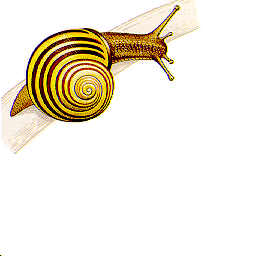
\includegraphics[width=5cm]{figuras/snail.png}
  \fonte{Adaptada de \url{https://people.math.sc.edu/Burkardt/data/bmp/bmp.html}.}
\end{figure}

\section{Métricas de avaliação}

As seguintes métricas foram consideradas:
\begin{itemize}
  \item \textbf{Taxa de compressão}: percentual do tamanho original após a compressão (quanto menor, melhor).
  \item \textbf{Tempo de compressão/descompressão}: medido em segundos.
  \item \textbf{Memória pico}: memória máxima observada durante a execução (MB).
  \item \textbf{Integridade}: verificação de \emph{round trip} (\texttt{decode(encode(x)) == x}).
\end{itemize}

\section{Resultados do LZ77 na \textit{Komm}}

A implementação do \textit{LZ77} na \textit{Komm} foi avaliada variando-se o tamanho da janela deslizante \(W\) (4\,kB a 64\,kB). As Figuras~\ref{fig:komm-alice-compression}–\ref{fig:komm-alice-time} apresentam os resultados sobre o texto \textit{Alice}; as Figuras~\ref{fig:komm-smiley-compression}–\ref{fig:komm-smiley-time}, sobre a imagem \textit{smiley}. Nos gráficos em que aparecem outros algoritmos, eles desempenham o papel de referência.

\begin{figure}[htp]
  \centering
  \caption{Texto \textit{Alice}: taxa de compressão (menor é melhor).}
  \label{fig:komm-alice-compression}
  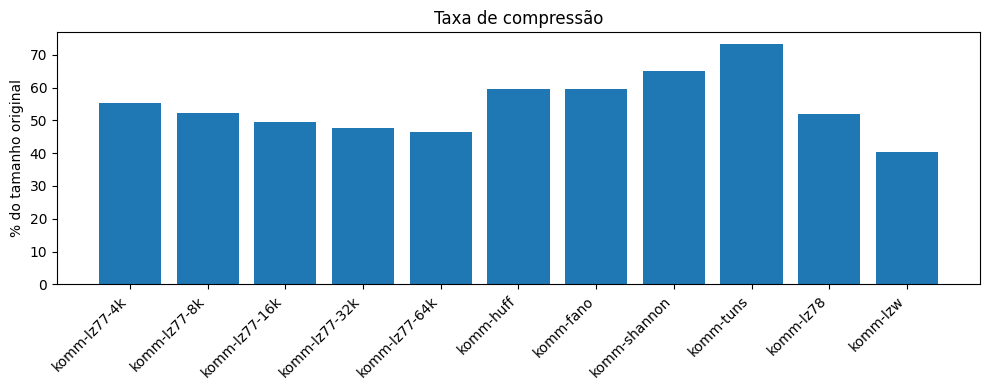
\includegraphics[width=15cm]{figuras/komm_alice_compression.png}
  \fonte{Elaborada pelo autor.}
\end{figure}

\begin{figure}[htp]
  \centering
  \caption{Texto \textit{Alice}: memória pico.}
  \label{fig:komm-alice-memory}
  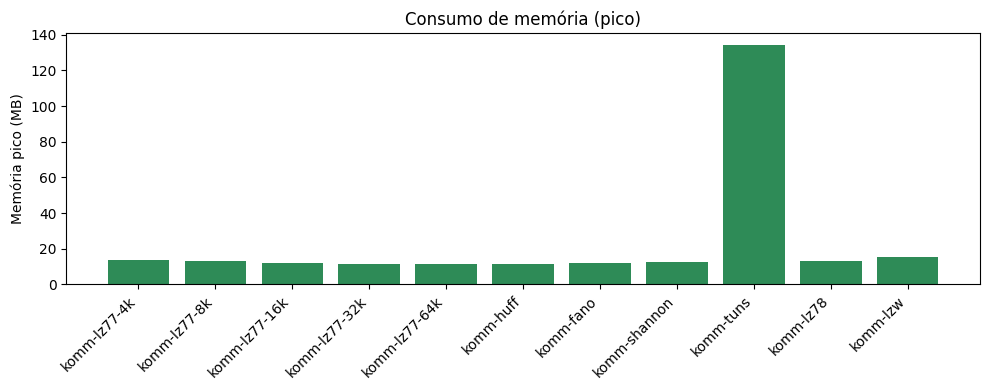
\includegraphics[width=15cm]{figuras/komm_alice_memory.png}
  \fonte{Elaborada pelo autor.}
\end{figure}

\begin{figure}[htp]
  \centering
  \caption{Texto \textit{Alice}: tempo de compressão.}
  \label{fig:komm-alice-time}
  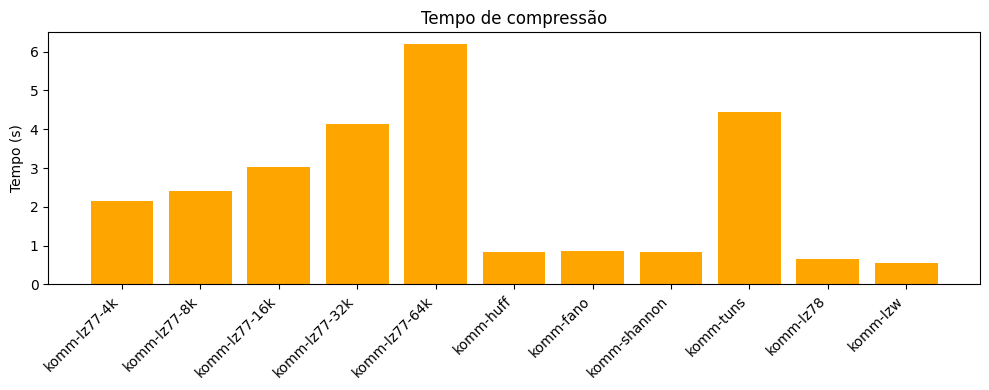
\includegraphics[width=15cm]{figuras/komm_alice_time.png}
  \fonte{Elaborada pelo autor.}
\end{figure}

\noindent\textbf{Observações (texto).}
\begin{itemize}
  \item O \textit{LZ77} apresenta o \emph{trade-off} esperado: aumentar \(W\) melhora a taxa de compressão (maior chance de \emph{matches} longos), ao custo de maior tempo e memória.
  \item Em relação às linhas de base, Huffman e Shannon--Fano são sistematicamente mais rápidos e leves, porém com taxas típicas de códigos prefixos; já Tunstall/LZ78/LZW situam-se entre os extremos.
\end{itemize}

\begin{figure}[htp]
  \centering
  \caption{Imagem \textit{smiley}: taxa de compressão (menor é melhor).}
  \label{fig:komm-smiley-compression}
  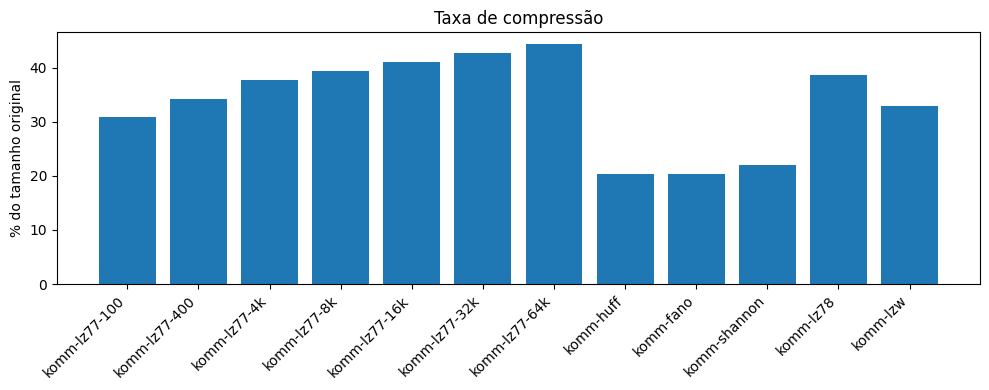
\includegraphics[width=15cm]{figuras/komm_smiley_compression.png}
  \fonte{Elaborada pelo autor.}
\end{figure}

\begin{figure}[htp]
  \centering
  \caption{Imagem \textit{smiley}: memória pico.}
  \label{fig:komm-smiley-memory}
  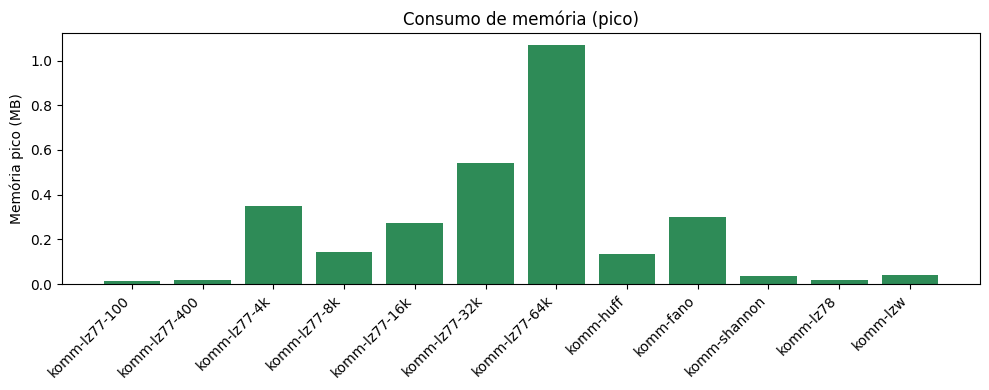
\includegraphics[width=15cm]{figuras/komm_smiley_memory.png}
  \fonte{Elaborada pelo autor.}
\end{figure}

\begin{figure}[htp]
  \centering
  \caption{Imagem \textit{smiley}: tempo de compressão.}
  \label{fig:komm-smiley-time}
  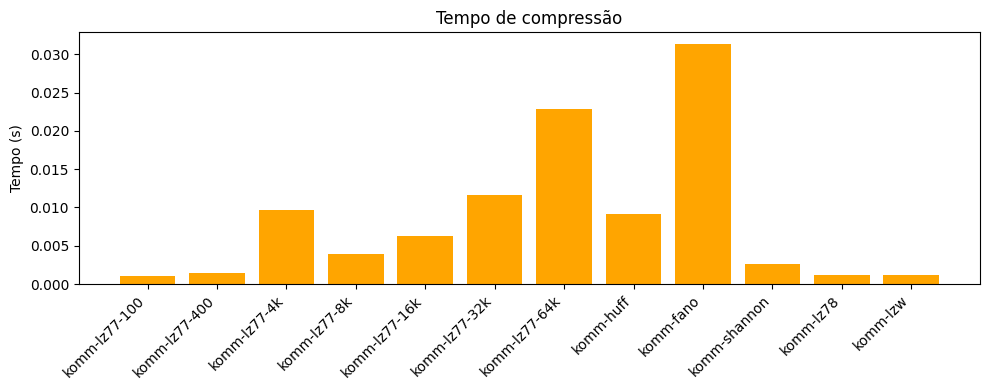
\includegraphics[width=15cm]{figuras/komm_smiley_time.png}
  \fonte{Elaborada pelo autor.}
\end{figure}

\noindent\textbf{Observações (imagem).}
\begin{itemize}
  \item Em imagens com grandes áreas uniformes, a variação de \(W\) também impacta: janelas maiores tendem a reduzir a taxa, porém com aumento de custo computacional.
  \item O benefício em taxa para imagens foi menos pronunciado que para texto, o que reflete a estrutura estatística distinta das fontes.
\end{itemize}

\begin{quadro}[htp]
\caption{Tempo de execução e pico de memória na imagem \textit{smiley} (implementações na \textit{Komm}).}\label{quadro:resultados-komm-smiley}
\begin{tabular}{|l|r|r|}
    \hline
    \textbf{Algoritmo de compressão} & \textbf{Tempo (s)} & \textbf{Pico de memória (MB)} \\
    \hline
    komm-lz77-4k   & 0,0096 & 367,894  \\ \hline
    komm-lz77-8k,97 & 0,0039 & 148,218  \\ \hline
    komm-lz77-16k  & 0,0062 & 287,370  \\ \hline
    komm-lz77-32k  & 0,0115 & 566,106  \\ \hline
    komm-lz77-64k  & 0,0228 & 112,2954 \\ \hline
    komm-huff      & 0,0092 & 140,961  \\ \hline
    komm-fano      & 0,0313 & 314,210  \\ \hline
    komm-shannon   & 0,0026 & 38,195   \\ \hline
    komm-tuns      & 3,750  & 15.1985,336 \\ \hline
    komm-lz78      & 0,0011 & 19,928   \\ \hline
    komm-lzw       & 0,0011 & 43,084   \\ \hline
\end{tabular}
\fonte{Elaborada pelo autor.}
\end{quadro}

\pagebreak
\pagebreak
\pagebreak

\section{Comparação com implementações externas de LZ77}\label{sec:externas}

Foram consideradas duas implementações populares: \textbf{FastLZ} (C) e \textbf{LZ77-Compressor} (Python). As configurações efetivas foram: \(W=8\,\text{KiB}\) e \(L=264\) bytes no \textit{FastLZ}; no \textit{LZ77-Compressor}, \(W\) variou entre 100 e 400 bytes e \(L=15\) bytes. Na \textit{Komm}, \(W\) e \(L\) são parametrizáveis; para comparação, utilizaram-se configurações próximas às disponíveis nas bibliotecas externas quando pertinente, além de uma configuração de referência com \(W=64\,\text{kB}\).

As Figuras~\ref{fig:external-alice-compression}–\ref{fig:external-alice-time} apresentam os resultados sobre o texto \textit{Alice}; as Figuras~\ref{fig:external-smiley-compression}–\ref{fig:external-smiley-time}, sobre a imagem \textit{smiley}.

\begin{figure}[htp]
  \centering
  \caption{Texto \textit{Alice}: taxa de compressão (menor é melhor).}
  \label{fig:external-alice-compression}
  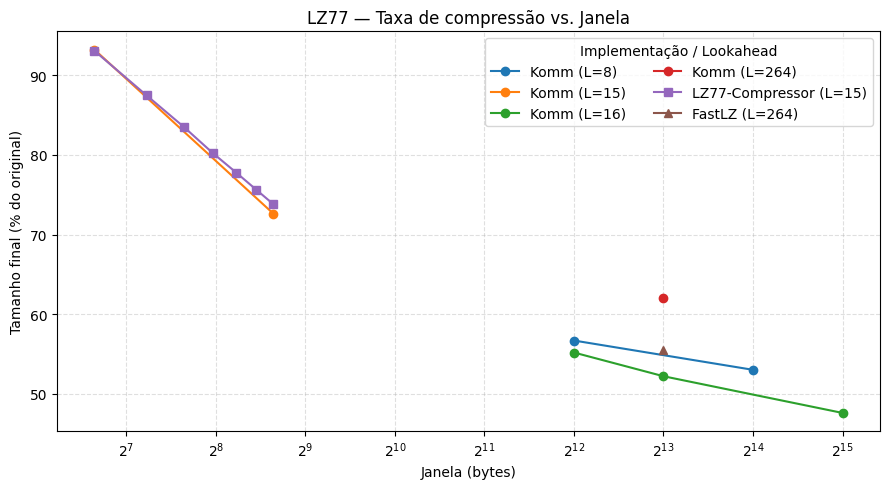
\includegraphics[width=15cm]{figuras/lz77_alice_compression_window.png}
  \fonte{Elaborada pelo autor.}
\end{figure}

\begin{figure}[htp]
  \centering
  \caption{Texto \textit{Alice}: memória pico.}
  \label{fig:external-alice-memory}
  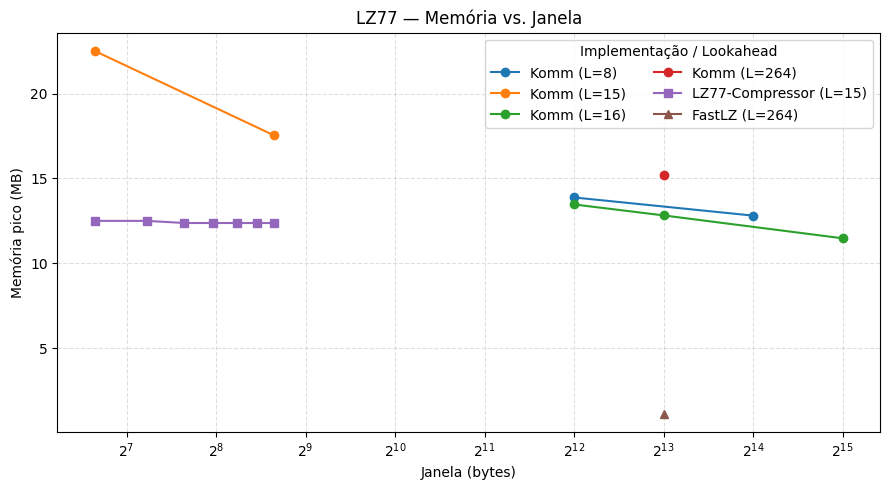
\includegraphics[width=15cm]{figuras/lz77_alice_memory_window.png}
  \fonte{Elaborada pelo autor.}
\end{figure}

\begin{figure}[htp]
  \centering
  \caption{Texto \textit{Alice}: tempo de compressão.}
  \label{fig:external-alice-time}
  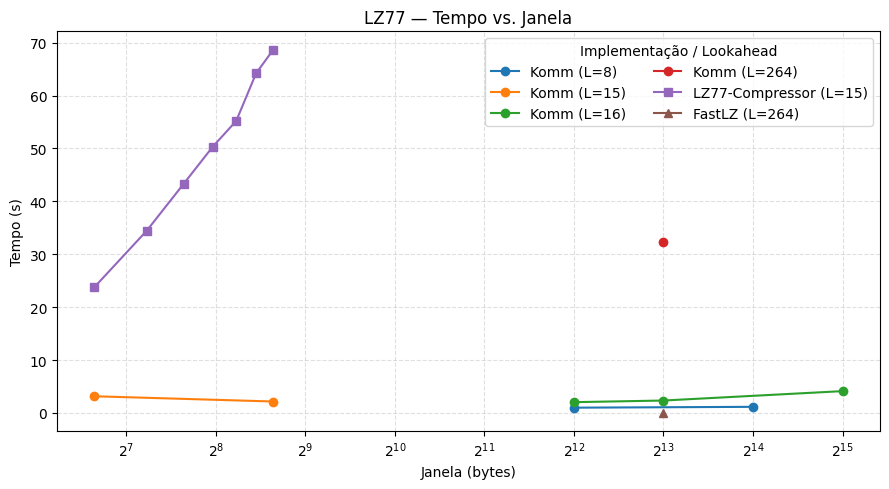
\includegraphics[width=15cm]{figuras/lz77_alice_time_window.png}
  \fonte{Elaborada pelo autor.}
\end{figure}

\noindent\textbf{Síntese (texto).}
\begin{itemize}
  \item \textit{FastLZ} obteve tempos inferiores, como esperado para uma implementação em C orientada a velocidade; em taxa, aproxima-se das melhores configurações do \textit{LZ77} na \textit{Komm} quando \(W\) é grande.
  \item \textit{LZ77-Compressor} apresentou maior tempo de execução, mas com consumo de memória contido para janelas pequenas.
\end{itemize}

\begin{figure}[htp]
  \centering
  \caption{Imagem \textit{smiley}: taxa de compressão (menor é melhor).}
  \label{fig:external-smiley-compression}
  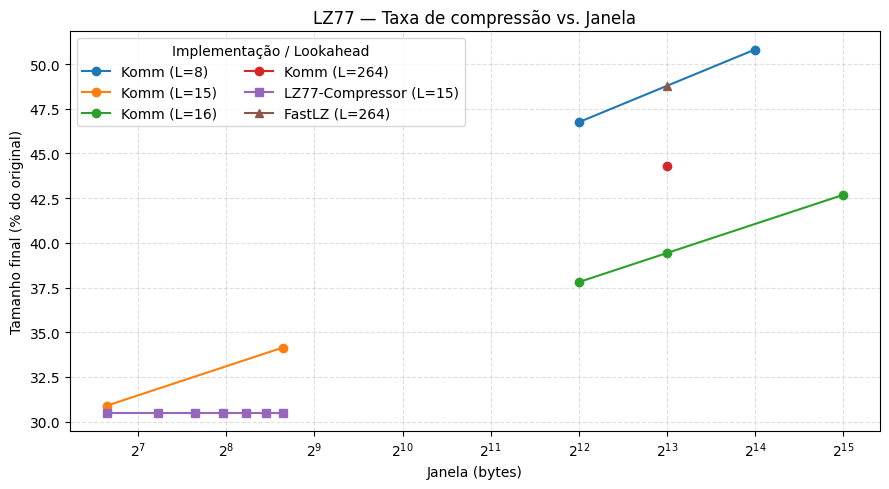
\includegraphics[width=15cm]{figuras/lz77_smiley_compression_window.png}
  \fonte{Elaborada pelo autor.}
\end{figure}

\begin{figure}[htp]
  \centering
  \caption{Imagem \textit{smiley}: memória pico.}
  \label{fig:external-smiley-memory}
  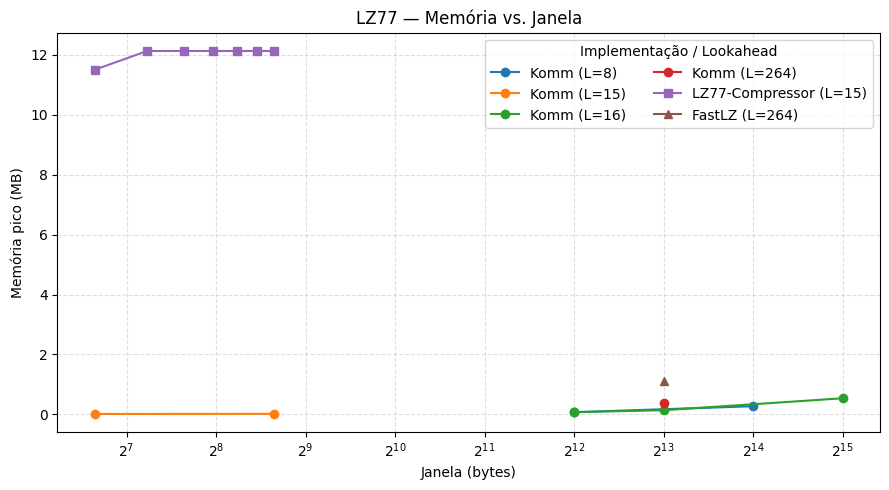
\includegraphics[width=15cm]{figuras/lz77_smiley_memory_window.png}
  \fonte{Elaborada pelo autor.}
\end{figure}

\begin{figure}[htp]
  \centering
  \caption{Imagem \textit{smiley}: tempo de compressão.}
  \label{fig:external-smiley-time}
  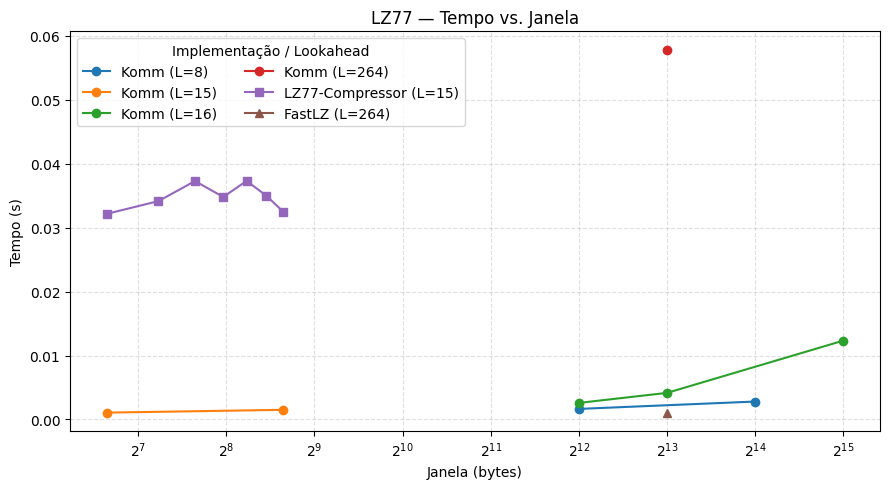
\includegraphics[width=15cm]{figuras/lz77_smiley_time_window.png}
  \fonte{Elaborada pelo autor.}
\end{figure}

\noindent\textbf{Síntese (imagem).}
\begin{itemize}
  \item A implementação da \textit{Komm} com janelas maiores superou as variantes externas em taxa de compressão na imagem \textit{smiley}.
  \item O \textit{FastLZ} manteve vantagem em tempo de execução.
  \item O \textit{LZ77-Compressor} permaneceu com tempos mais altos; o uso de memória variou conforme o tamanho de janela.
\end{itemize}

\section{Discussão}

Os resultados confirmam os compromissos clássicos do \textit{LZ77}: (i) janelas maiores favorecem taxas menores (melhor compressão) em fontes com repetições de longo alcance; (ii) o custo em tempo e memória cresce com \(W\); (iii) implementações em C orientadas a desempenho tendem a dominar em tempo, enquanto a versão modular na \textit{Komm} privilegia clareza, reprodutibilidade e integração com os demais módulos da biblioteca. Todas as execuções passaram no teste de integridade (\emph{round trip}).
